
%(BEGIN_QUESTION)
% Copyright 2006, Tony R. Kuphaldt, released under the Creative Commons Attribution License (v 1.0)
% This means you may do almost anything with this work of mine, so long as you give me proper credit

Shown here are three different cages from cage-guided globe valves.  Identify the respective flow characteristic ({\it linear}, {\it equal percentage}, or {\it quick opening}) for each cage shown here:

$$\includegraphics[width=15.5cm]{i01383x01.eps}$$

\underbar{file i01383}
%(END_QUESTION)





%(BEGIN_ANSWER)

$$\includegraphics[width=15.5cm]{i01383x02.eps}$$
 
%(END_ANSWER)





%(BEGIN_NOTES)

Identifying the opening characteristics for valve cages is a little different than identifying characteristics by plug shape.  Whereas the plug shape represented how much the seat throat would be {\it blocked} by the plug, the ``window'' shapes in a cage represent how much the valve will be {\it open} to flow as the piston-shaped plug rises to uncover more of the window area.

\vskip 10pt

The {\it quick opening} cage is fairly easy to identify: the window ``opens'' quickly as the plug rises to uncover its area.

\vskip 10pt

The {\it linear cage} looks like a ``stepped'' version of the quick opening cage, but is rectangular throughout most of its shape.  Equal changes in plug rise will uncover equal amounts of area in the window.  The larger window area uncovered at the end of the plug's travel is necessary to compensate for the effect of ``diminishing returns'' with regard to the tortuous flow path through the globe valve body.  To put it simply, the cage ports {\it must} become wider near the top in order to maintain a linear $C_v$/opening characteristic because the plug becomes less influential on flow at high percentages of opening.

\vskip 10pt

In the {\it equal percentage} cage, the window is tapered toward the bottom.  This results in an exponential increase in uncovered window area as the plug rises (slow at first, but becoming faster with additional increases in plug motion).

\vskip 10pt

Photographs of characterized cages may generally be found in valve sales brochures.  The Fisher ``Easy-E'' globe-style control valve product flier, for example, provides pictures of the three major cage characteristics available.

%INDEX% Final Control Elements, valve: characterization

%(END_NOTES)


